 \documentclass [12pt]{article} 

\usepackage {amsmath}
\usepackage {amsthm}
\usepackage {amssymb}
\usepackage {graphicx} 
\usepackage {float}
\usepackage {multirow}
\usepackage {xcolor}
\usepackage {algorithmic}
\usepackage [ruled,vlined,commentsnumbered,titlenotnumbered]{algorithm2e} \usepackage {array} 
\usepackage {booktabs} 
\usepackage {url} 
\usepackage {parskip} 
\usepackage [margin=1in]{geometry} 
\usepackage [T1]{fontenc} 
\usepackage {cmbright} 
\usepackage [many]{tcolorbox} 
\usepackage [colorlinks = true,
            linkcolor = blue,
            urlcolor  = blue,
            citecolor = blue,
            anchorcolor = blue]{hyperref} 
\usepackage {enumitem} 
\usepackage {xparse} 
\usepackage {verbatim}
\usepackage{listings}
\usepackage{xcolor}
\lstset { %
    language=C++,
    backgroundcolor=\color{black!5}, % set backgroundcolor
    basicstyle=\footnotesize,% basic font setting
}
\newtheorem{theorem}{Theorem}
\newtheorem{remark}{Remark}
\newtheorem{lemma}[theorem]{Lemma}
\theoremstyle{definition}
\newtheorem{definition}{Definition}[section]



\DeclareTColorBox {Solution}{}{breakable, title={Solution}} \DeclareTColorBox {Solution*}{}{breakable, title={Solution (provided)}} \DeclareTColorBox {Instruction}{}{boxrule=0pt, boxsep=0pt, left=0.5em, right=0.5em, top=0.5em, bottom=0.5em, arc=0pt, toprule=1pt, bottomrule=1pt} \DeclareDocumentCommand {\Expecting }{+m}{\textbf {[We are expecting:} #1\textbf {]}} \DeclareDocumentCommand {\Points }{m}{\textbf {(#1 pt.)}} 

\begin {document} 

\vspace {1em} 
\begin {Instruction} 
Adapted From Virginia Williams' lecture notes.
\end {Instruction}  

{\LARGE \textbf {COMP 285 (NC A\&T, Spr `22)}\hfill \textbf {Lecture 18} } 

\begin{centering}
\section*{Strongly Connected Components}
\end{centering}
 
 \section{Connected components in undirected graphs} 

 A connected component of an undirected graph $ G = (V, E)$ is a maximal set of vertices $S \subset V$ such that for each $u \in S$ and $v \in S$, there exists a path in $G$ from vertex $u$ to vertex $v$.

\begin{definition}[Formal Definition]
Let $u \equiv v$ if and only if $G$ has a path from vertex $u$ to vertex $v$ . This is an equivalence relation (it is symmetric, reflexive, and transitive). Then, a connected component of $G$ is an equivalence class of this relation $\equiv$. Recall that the equivalence class of a vertex $u$ over a relation $\equiv$ is the set of all vertices $v$ such that $u \equiv v$.
\end{definition}

 \subsection{Algorithm to find connected components in a undirected graph}

In order to find a connected component of an undirected graph, we can just pick a vertex and start doing a search (BFS or DFS) from that vertex. All the vertices we can reach from that vertex compose a single connected component. To find all the connected components, then, we just need to go through every vertex, finding their connected components one at a time by searching the graph. Note however that we do not need to search from a vertex v if we have already found it to be part of a previous connected component. Hence, if we keep track of what vertices we have already encountered, we will only need to perform one BFS for each connected component.


\begin{proof}
When searching from a particular vertex v , we will clearly never reach any nodes outside the connected component with DFS or BFS. So we just need to prove that we will in fact reach all connected vertices. We can prove this by induction: Consider the vertices at minimum distance $i$ from vertex $v$. Call these vertices ``level $i$'' vertices. If BFS or DFS successfully reaches all vertices at level $i$, then they must reach all vertices at level $i + 1$, since each vertex at distance $i + 1$ from v must be connected to some vertex at distance $i from v$ . This is the inductive step, and for the base case, DFS or BFS will clearly reach all vertices at level $0$ (just v itself). So indeed this algorithm will find each connected component correctly.
\end{proof}

The searches in the above algorithm take total time $O(|E| + |V |),$ because each BFS or DFS call takes linear time in the number of edges and vertices for its component, and each component is only searched once, so all searches will take time linear in the total number of edges and vertices.

\begin{figure}[h!]
\centering
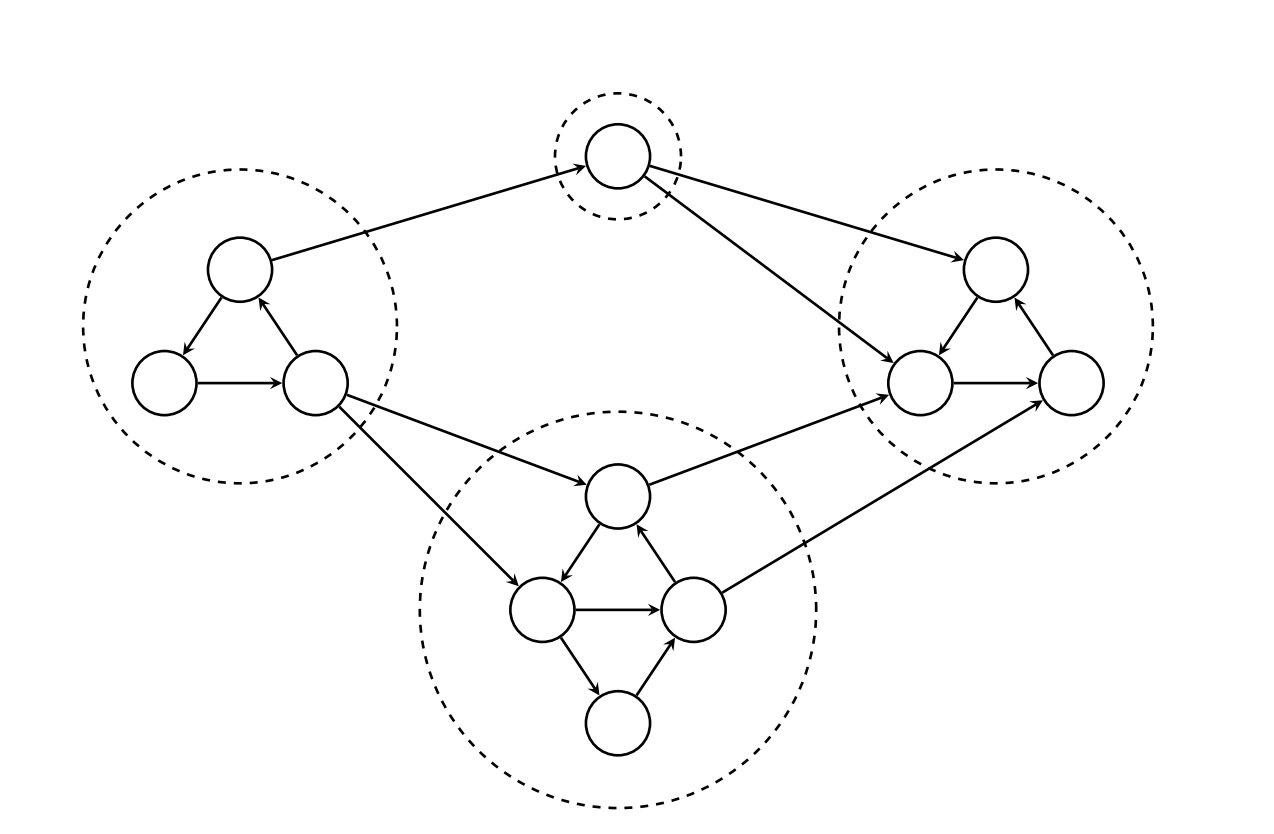
\includegraphics[scale=0.5]{scc_graph.png}
\caption{The strongly connected components of a directed graph}
\label{fig:scc_graph}
\end{figure}

\section{Connectivity in directed graphs}
How can we extend the notion of connected components to directed graphs?

\begin{definition}[Strongly connected component (SCC)]
A strongly connected component in a directed graph $G = (V, E)$ is a maximal set of vertices $S \subset V$ such that each vertex $v \in S$ has a path to each other vertex $u \in S$. This is the same as the definition using equivalence classes for undirected graphs, except now $u \equiv v$ if and only if there is a path from $u$ to $v$ AND a path from $v$ to $u$.
\end{definition}

\begin{definition}[Weakly connected compnent]
Let $G = (V, E)$ be a directed graph, and let $G'$ be the undirected graph that is formed by replacing each directed edge of $G$ with an undirected edge. Then the weakly connected components of $G$ are exactly the connected components of $G'$.
\end{definition}

\section{Algorithm to find strongly connected components of a directed graph}

The algorithm we present is essentially two passes of depth-first search, plus some extremely clever additional book-keeping. The algorithm is described in a top-down fashion in Algorithms \ref{alg:1} to \ref{alg:3}. Algorithm \ref{alg:1} describes the top level of the algorithm, and Algorithm \ref{alg:2} and Algorithm \ref{alg:3} describe the subroutines DFS-Loop and DFS. Read these procedures carefully before proceeding to the next section.

\begin{algorithm}
\caption{The top level of our SCC algorithm. The $f$-values and leaders are computed in the first and second calls to DFS-Loop, respectively (see below)}
\label{alg:1}
\begin{algorithmic}
\STATE \textbf{INPUT:} A directed graph $G = (V,E)$, in adjacency list representation. Assume that the vertices $V$ are labeled $1, 2, 3, \cdots, n$.
\STATE $G^{\text{rev}} \gets$ the graph $G$ after the orientation of all arcs have been reversed.
\STATE Run the DFS-Loop subroutine on $G^{\text{rev}}$, processing vertices in any arbitrary order, to obtain a finishing time $f(v)$ for each vertex $v \in V$.
\STATE Run the DFS-Loop subrouting on $G$, processing vertices in creasing order of $f(v)$, to assign a ``leader'' to each vertex $v \in V$. The leader of a vertex $v$ will be the source vertex that the DFS that discovered $v$ started from.
\STATE The strongly connected components of $G$ correspond to vertices of $G$ that share a common leader.
\end{algorithmic}
\end{algorithm}

\begin{algorithm}
\caption{The DFS-Loop subroutine}
\label{alg:2}
\begin{algorithmic}
\STATE \textbf{INPUT:} A directed graph $G = (V,E)$, in adjacency list representation.
\STATE Let global variable $t \gets 0$ \texttt{/* This keeps track of the number of vertices that have been fully explored */}
\STATE Let global variable $s \gets $NULL \texttt{/* This keeps track of the vertex from which the last DFS call was invoked */}
\FOR{$i = n, n-1, \cdots, 1$}
    \STATE \texttt{// In the first call, vertices are labeled $1, 2, \cdots, n$ arbitrarily. In the second call, vertices are labeled by their $f(v)$-values from the first call.}
    \IF{$i$ not yet explored}
        \STATE Let $s \gets i$ \texttt{/* Set the current source $s$ to $i$ All vertices discovered from the below DFS call will have their leaders set to $s$ */}
        \STATE DFS(G, i)
    \ENDIF
\ENDFOR
\end{algorithmic}
\end{algorithm}


\begin{algorithm}
\caption{The DFS subroutine. The $f$-values only need to be computed during the first call to DFS-Loop, and the ledaer values only need to be computed during the second call to DFS-Loop.}
\label{alg:3}
\begin{algorithmic}
\STATE \textbf{INPUT:} A directed graph $G = (V,E)$, in adjacency list representation, and source vertex $i \in V$.
\STATE Mark $i$ as explored. \texttt{/* It remains explored for the entire duration of the DFS-Loop call */}
\STATE leader($i) \gets s$
\FOR{arc($i,j$) in $G$}
    \IF{$j$ noto yet explored}
        \STATE DFS($G,j$)
    \ENDIF
\ENDFOR
\STATE $t \gets t + 1$
\STATE Let $f(i) \gets t$
\end{algorithmic}
\end{algorithm}

\begin{remark} 
The algorithm in Algorithm \ref{alg:1} is a bit different than the one in CLRS/Lecture! The difference is that in these notes, we first run DFS on the reversed graph, and then we run it again on the original; in CLRS, we first run DFS on the original, and then the second time on the reversed graph. Is it the case that one of these two textbooks has messed it up? In fact, it doesn't matter: the SCCs of$G$ are the same as the SCCs of $G^{\text{rev}}$ , so both algorithms find exactly the same SCC decomposition.
\end{remark} 

As we've seen, each invocation of DFS-Loop can be implemented in linear time (i.e., $O(|E|+ |V |)$), so this whole algorithm will take linear time (the bookkeeping of leaders and finishing times just adds a constant number of operations per each node).

\section{An Example}
 
But why on earth should this algorithm work? An example should increase its plausibility (though it certainly doesn't constitute a proof of correctness). Figure \ref{fig:g_rev_scc} displays a reversed graph $G^{\text{rev}}$, with its vertices numbered arbitrarily, and the $f$-values computed in the first call to DFS-Loop. In more detail, the first DFS is initiated at node $9$. The search must proceed next to node $6$. DFS then has to make a choice between two different adjacent nodes; we have shown the $f$-values that ensue when DFS visits node $3$ before node $8$.\footnote{Different choices of which node to visit next generate different sets of $f$-values, but our proof of correctness will apply to all ways of resolving these choices}. When DFS visits node $3$ it gets stuck; at this point node $3$ is assigned a finishing time of $1$. DFS backtracks to node $6$, proceeds to node $8$, then node $2$, and then node $5$. DFS then backtracks all the way back to node $9$, resulting in nodes $5, 2, 8, 6$, and $9$ receiving the finishing times $2, 3, 4, 5$, and $6$, respectively. Execution returns to DFS-Loop, and the next (and final) call to DFS begins at node $7$.

\begin{figure}[h!]
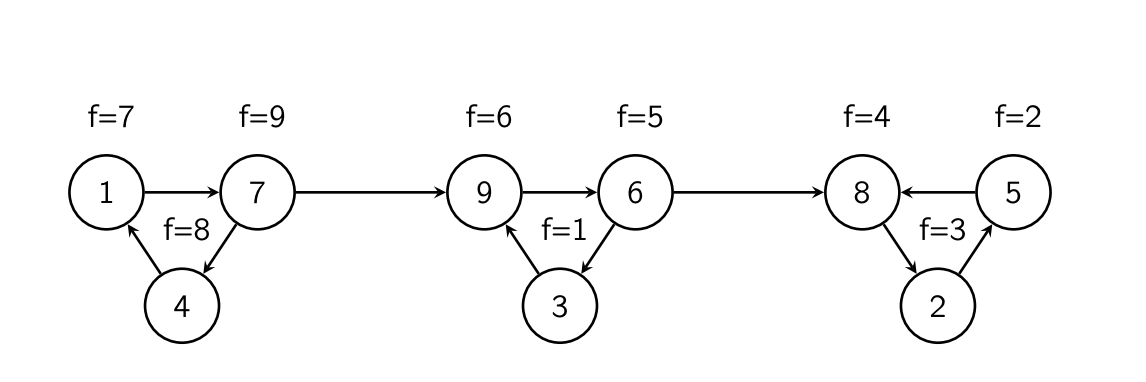
\includegraphics[scale=0.8]{g_rev_scc.png}
\caption{Example exuection of the strongly connected components algorithm. Nodes tare labaled arbitrarily and their finishing times are shown.}
\label{fig:g_rev_scc}
\end{figure}

\begin{figure}[h!]
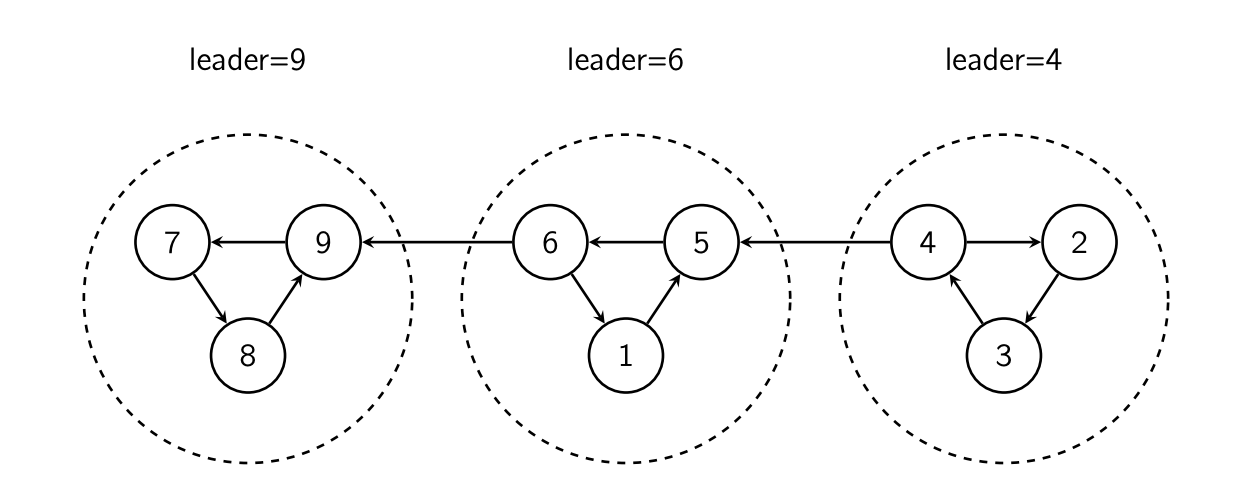
\includegraphics[scale=0.8]{scc_alg.png}
\caption{Example execution of the strongly connected components algorithm. Nodes are labeled by their finishing times and their leaders are shown.}
\label{fig:scc_alg}
\end{figure}

Figure \ref{fig:scc_alg} shows the original graph (with all arcs now unreversed), with nodes labeled withtheir finishing times. The magic of the algorithm is now evident, as the SCCs of $G$ present themselves to us in order: since we call DFS on the nodes in decreasing order of their finishing times, the first call to DFS discovers the nodes 7-9 (with leader 9); the second the nodes 1,5, and 6 (with leader 6); and the third the remaining three nodes (with leader 4).

\subsection{The Acyclic Meta-Graph of SCCs} 
First, observe that the strongly connected components of a directed graph form an acyclic ``meta-graph'', where the meta-nodes correspond to the SCCs $C_1, \cdots , C_k$ , and there is an arc $C_h \to C_{\ell}$ with $h \neq \ell$ if and only if there is at least one arc $(i, j)$ in $G$ with $i \in C_h$ and $j \in C_{\ell}$. This directed graph must be acyclic: since within a SCC you can get from anywhere to anywhere else on a directed path, in a purported directed cycle of SCCs you can get from every node in a constituent SCC to every other node of every other SCC in the cycle. Thus the purported cycle of SCCs is actually just a single SCC. Summarizing, every directed graph has a useful ``two-tier'' structure: zooming out, one sees a DAG (Directed Acyclic Graph) on the SCCs of the graph; zooming in on a particular SCC exposes its finer-grained structure. For example, the meta-graphs corresponding to the directed graphs in Figs. \ref{fig:scc_graph} and \ref{fig:scc_alg} are shown in Fig. \ref{fig:meta_graph_scc}.

\begin{figure}
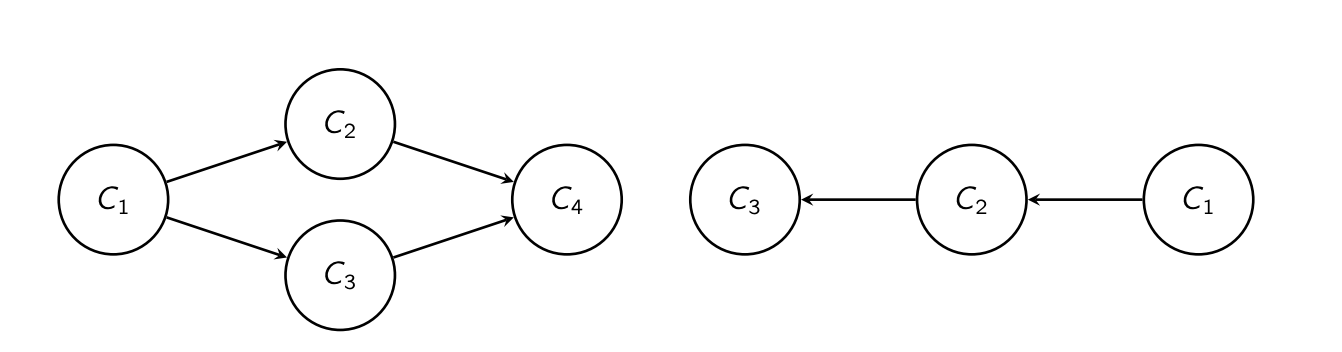
\includegraphics[scale=0.8]{meta_graph_scc.png}
\caption{The DAGs of the SCCs of the graphs in Figs. \ref{fig:scc_graph} and \ref{fig:scc_alg}.}
\label{fig:meta_graph_scc}
\end{figure}

\section{Proof of Correctness}
\subsection{The Key Lemma}
Correctness of the algorithm hinges on the following key lemma.

\begin{lemma} 
Consider two ``adjacent'' strongly connected components of a graph $G$: components $C_1$ and $C_2$ such that there is an arc $(i, j)$ of $G$ with $i \in C_1$ and $j \in C_2$. Let $ f (v )$ denote the finishing time of vertex $v$ in some execution of DFS-Loop on the reversed graph $G^{\text{rev}}$. Then
$$
\max_{v\in C_1} f(v) < \max_{v\in C_2}f(v)
$$
\end{lemma}

\begin{proof} 
Consider two adjacent SCCs $C_1$ and $C_2$, as they appear in the reversed graph $G^{\text{rev}}$ - where there is an arc $(j, i)$, with $j \in C_2$ and $i \in C_1$ (Fig. \ref{fig:scc_proof}). Because the equivalence relation defining the SCCs is symmetric, G and $G^{\text{rev}}$ have the same SCCs; thus $C_1$ and $C_2$ are also SCCs of $G^{\text{rev}}$. Let $v$ denote the first vertex of $C_1 \cup C_2$ visited by DFS-Loop in $G^{\text{rev}}$. There are now two cases. 

First, suppose that $v \in C_1$ (Fig. \ref{fig:scc_proof}). Since there is no non-trivial cycle of SCCs (Section 4.1), there is no directed path from $v$ to $C_2$ in $G^{\text{rev}}$. Since DFS discovers everything reachable and nothing more, it will finish exploring all vertices in $C_1$ without reaching any vertices in $C_2.$ Thus, every finishing time in $C_1$ will be smaller that every finishing time in $C_2$, and this is even stronger than the assertion of the lemma. (Cf., the left and middle SCCs in Fig. \ref{fig:scc_alg}.) Second, suppose that $v \in C_2$ (Fig. \ref{fig:scc_proof}). Since DFS discovers everything reachable and nothing more, the call to DFS at $v$ will finish exploring all of the vertices in $C_1 \cup C_2$ before ending. Thus, the finishing time of $v$ is the largest amongst vertices in $C_1 \cup C_2$, and in particular is larger than all finishing times in $C_1$. (Cf., the middle and right SCCs in Fig. \ref{fig:scc_alg}.)

This completes the proof.
\end{proof}

\begin{figure}
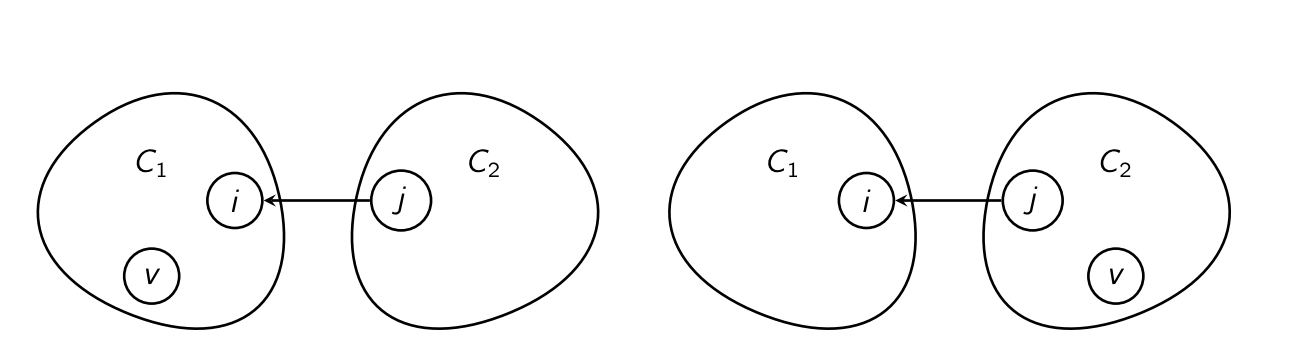
\includegraphics[scale=0.8]{scc_proof.png}
\caption{Proof of key lemma. Vertex $v$ is the first in$ C_1 \cup C_2$ visited during the execution of DFS-Loop on $G^{\text{rev}}$. On the left, all $f$-values in $C_1$ smaller than in $C_2$. On the right: $v$ has the largest $f$-value in $C_1 \cup C_2$.}
\label{fig:scc_proof}
\end{figure}

\subsection{The Final Argument} 

The Key Lemma says that traversing an arc from one SCC to another (in the original, unreversed graph) strictly increases the maximum $f$-value of the current SCC. For example, if $f_i$ denotes the largest $f$-value of a vertex in $C_i$ in Fig. \ref{fig:meta_graph_scc}, then we must have $f_1 < f_2, f_3 < f_4$. Intuitively, when DFS-Loop is invoked on $G$, processing vertices in decreasing order of finishing times, the successive calls to DFS peel off the SCCs of the graph one at a time, like layers of an onion. 

We now formally prove correctness of our algorithm for computing strongly connected components. Consider the execution of DFS-Loop on $G$. We claim that whenever DFS is called on a vertex $v$, the vertices explored - and assigned a common leader - by this call are precisely those in $v$'s SCC in $G$. Since DFS-Loop eventually explores every vertex, this claim implies that the SCCs of $G$ are precisely the groups of vertices that are assigned a common leader. 

We proceed by induction. Let $S$ denote the vertices already explored by previous calls to DFS (initially empty). Inductively, the set $S$ is the union of zero or more SCCs of G. Suppose DFS is called on a vertex $v$ and let $C$ denote $v$'s SCC in $G$. Since the SCCs of a graph are disjoint, $S$ is the union of SCCs of G, and $v \notin S$, no vertices of $C$ lie in $S$. Thus, this call to DFS will explore, at the least, all vertices of $C$. By the Key Lemma, every outgoing arc $(i, j)$ from $C$ leads to some SCC $C'$ that contains a vertex w with a finishing time larger than $f (v)$. Since vertices are processed in decreasing order of finishing time, $w$ has already been explored and belongs to $S$; since $S$ is the union of SCCs, it must contain all of $C'$ . Summarizing, every outgoing arc from $C$ leads directly to a vertex that has already been explored. Thus this call to DFS explores the vertices of $C$ and nothing else. This completes the inductive step and
the proof of correctness.
\end{document}